\documentclass[10pt]{article}
\usepackage{graphicx,amsmath, bm, verbatim, comment, amssymb}
\usepackage[margin=1in]{geometry}

\usepackage{hyperref}

\parindent 0.25 in

\begin{document}
\vspace*{0.05\textheight}

\begin{center}

\begin{Huge} \underline{\textbf{infraGA/GeoAc}} \end{Huge}

\vspace*{0.025\textheight}

\begin{Large}
\underline{Numerical tools to model infrasonic propagation} \\
\vspace*{5pt}

\underline{in the limit of geometric acoustics}
\end{Large}

\vspace*{0.05\textheight}

\textit{Author/Maintainer: Philip S. Blom (pblom@lanl.gov)}

\end{center}

\vfill

\begin{flushleft}
\begin{footnotesize}

Copyright \copyright \, 2014, Triad National Security, LLC 

\vspace{5pt}

All rights reserved.

\vspace{5pt}

Copyright 2014. Triad National Security, LLC. This software was produced under U.S. Government contract DE-AC52-06NA25396 for Los Alamos National Laboratory (LANL), which is operated by Triad National Security, LLC for the U.S. Department of Energy. The U.S. Government has rights to use, reproduce, and distribute this software.  NEITHER THE GOVERNMENT NOR TRIAD NATIONAL SECURITY, LLC MAKES ANY WARRANTY, EXPRESS OR IMPLIED, OR ASSUMES ANY LIABILITY FOR THE USE OF THIS SOFTWARE.  If software is modified to produce derivative works, such modified software should be clearly marked, so as not to confuse it with the version available from LANL.

\vspace{5pt}
 
Additionally, permission is hereby granted, free of charge, to any person obtaining a copy of this software and associated documentation files (the "Software"), to deal in the Software without restriction, including without limitation the rights to use, copy, modify, merge, publish, distribute, sublicense, and/or sell copies of the Software, and to permit persons to whom the Software is furnished to do so, subject to the following conditions:
 
 \vspace{5pt}

The above copyright notice and this permission notice shall be included in all copies or substantial portions of the Software.

\vspace{5pt}
 
THE SOFTWARE IS PROVIDED "AS IS", WITHOUT WARRANTY OF ANY KIND, EXPRESS OR IMPLIED, INCLUDING BUT NOT LIMITED TO THE WARRANTIES OF MERCHANTABILITY, FITNESS FOR A PARTICULAR PURPOSE AND NONINFRINGEMENT. IN NO EVENT SHALL THE AUTHORS OR COPYRIGHT HOLDERS BE LIABLE FOR ANY CLAIM, DAMAGES OR OTHER LIABILITY, WHETHER IN AN ACTION OF CONTRACT, TORT OR OTHERWISE, ARISING FROM, OUT OF OR IN CONNECTION WITH THE SOFTWARE OR THE USE OR OTHER DEALINGS IN THE SOFTWARE.
 
 \end{footnotesize}
\end{flushleft} 

\newpage

\tableofcontents

\newpage
\section{Introduction and Installation}
\label{Sect:Intro_Install}
\hspace*{0.25in}  InfraGA/GeoAc is a numerical package written in C++, which solves the equations governing acoustic propagation through the atmosphere in the geometric limit using the geometric acoustic methods in the GeoAc library via a classical fourth-order Runge Kutta (RK4) algorithm.  The toolkit contains multiple instances of said equation system and is able to model propagation in an azimuthal plane using the effective motionless medium approximation as well as in three dimensions using an inhomogeneous moving background medium.  The three dimensional propagation scheme include methods to model propagation in a Cartesian coordinate system as well as a curvilinear coordinate system which incorporates the curvature of the earth as either spherical or elliptical (as defined by the WGS84 ellipsoid). 

In addition to the geometric propagation paths which are straightforward to compute, the GeoAc library uses auxiliary parameters as discussed in \textit{Impulse propagation in the nocturnal boundary layer - analysis of the geometric component} [Blom \& Waxler; J. Acoust. Soc. Am., 2012, Vol.131(5), pp.3680--90] to calculate the Jacobian determinant and obtain a frequency independent amplitude coefficient describing the attenuation due to geometric spreading.  The auxiliary parameters used to compute the amplitude coefficient have been found to provide an efficient means to identify eigenrays (propagation paths connecting a source and receiver at specific locations) as detailed in \textit{Modeling and observations of an elevated, moving infrasonic source: eigenray methods} [Blom \& Waxler; J. Acoust. Soc. Am., 2016, In Review].  Eigenray information provides a means to predict the characteristics of the various acoustic phases observed at a given receiver location for a known source and propagation medium.

For propagation through a horizontally varying medium, a multivariate interpolation scheme has been developed which uses a modified Keys bicubic interpolation algorithm as described in \textit{Cubic Convolution Interpolation for Digital Image Processing}  [IEEE Transactions on Signal Processing, Acoustics, Speech, and Signal Processing 29 (6): pp.1153-60].  In this case, the interpolation algorithm has been configured so that both first and second order derivatives of the medium are continuous between grid squares.  This condition is required to generate smooth and continuous solutions for the auxiliary parameters used in computation the geometric spreading.

Topographical features can be incorporated into the propagation modeling, though the required interpolation precision significantly increases computation time.  Methods currently allow for topographical effects in a plane (using the effective sound speed approximation for the atmosphere) or for a full two dimensional topographical structure which produces significant non-planar propagation in the case of topographical gradients perpendicular to the azimuth of propagation.  Note that the topographical effects modeled in the geometric limit neglect diffraction and scattering.

\vspace*{10pt} 

\hspace{-0.25in}\textbf{Installation}:
 \begin{itemize}
   \item Ensure that dependencies are installed: \verb=fftw=, \verb=OpenMPI= (optional).
   \item Open a terminal, \verb=cd= into the directory containing the infraGA/GeoAc materials
   \item To create the standard methods within the local directory structure, run \verb=make=.
   \item If you have \verb=OpenMPI=, you can build the multi-threaded version of infraGA by running \verb=make accel=.
 \end{itemize}

The rest of this manual is divided up into the following sections:  explanation of the usage of the individual executables are detailed in the Sect. 2, clarification of the amplitude computation and range dependent profile interpolation are summarized in Sect. 3, details of additional parameters available for all executables to customize propagation are given in Sect. 4.  An overview of the changes made during each revision of the package are included in Sect. 5.

\newpage
\section{Using infraGA}
\label{Sect:Usage}

All of the methods in InfraGA have usage output that is displayed if no arguments are provided to the call.  These usage summaries have example usage calls that can be helpful in understanding how to run the code.  Additional details for each method are provided below.

\subsection{2D Stratified Cartesian Propagation}
\label{Sect:Usage:2D}
\textbf{Description}  

The methods in \verb=infraga-2d= compute ray paths in an azimuthal plane using the effective sound speed approximation.  These methods are useful for comparing predictions with other propagation schemes (normal mode, parabolic equation, etc.) that require the effective sound speed.

\vspace{0.02\textheight}

\hspace{-0.25in}\textbf{Usage} 

\begin{center} \begin{large}
\verb=infraga-2d  [option]  profile.met  [parameters]=
\end{large} \end{center}

\begin{itemize}
 \item Only one option can be applied for a given run.  Possible options are:

\begin{tabular}{  l l }
  \verb=-prop=		& Generate ray paths at a fixed azimuth using multiple inclination angles. \\
  \verb=-wnl_wvfrm=	& Compute the weakly non-linear waveform evolution along a single ray path.
 \end{tabular}
 
 \item The \verb=profile.met= file is expected to contain columns describing the atmosphere in the format:

\begin{equation*} 
 z \left[ \text{km} \right] \hspace{2pt} \vdots \hspace{2pt}
 T(z) \left[ \text{K} \right] \hspace{2pt} \vdots \hspace{2pt}
 u(z) \left[ \frac{\text{m}}{\text{s}} \right] \hspace{2pt} \vdots \hspace{2pt}
 v(z) \left[ \frac{\text{m}}{\text{s}} \right] \hspace{2pt} \vdots \hspace{2pt}
 \rho_0(z) \left[ \frac{\text{g}}{\text{cm}^3} \right] \hspace{2pt} \vdots \hspace{2pt}
 p_0(z) \left[ \text{mbar} \right] 
\end{equation*}

 \item Parameters are set using the format \verb#parameter_name=value#, for example: \verb#incl_step=1.0#.  Possible parameters for each option are included below.
 \end{itemize}

\begin{tabular}{ | l | l | c | }
  \hline
  \multicolumn{3}{|c|}{\textbf{Parameters for propagation option}} \\
  \hline
  Parameter & Description & Default Value \\
  \hline \hline
 \verb=incl_min= 		& Minimum inclination angle (0\(^o\) = horizontal)		& \(0.5^o\)	\\
 \verb=incl_max= 		& Maximum inclination angle (0\(^o\) = horizontal)		& \(45.0^o\) \\
 \verb=incl_step=  		& Inclination step size							& \(0.5^o\) \\ \hline
 \verb=azimuth=		& Azimuth angle (North = 0\(^o\), increases clockwise)	& \(-90.0^o\) \\ \hline
 \verb=bounces=		& Maximum \# of bounces to compute (integer \(\geq 0\)) 	& 2 \\ \hline
 \verb=src_alt=			& Altitude of the source (rel. sea level)				& 0.0 km \\ \hline
\end{tabular}

\vspace{0.02\textheight}

\begin{tabular}{ | l | l | c | }
  \hline
  \multicolumn{3}{|c|}{\textbf{Parameters for weakly non-linear waveform option}} \\
  \hline
  Parameter & Description & Default Value \\
 \hline \hline
 \verb=inclination=		& Initial inclination angle of the ray					& 10\(^o\) \\
 \verb=azimuth=		& Initial azimuth angle of the ray					& 90\(^o\) \\
 \verb=bounces=		& \# of bounces to compute (integer \(\geq 0\)) 			& 0 \\ \hline
 
 \verb=src_alt=			& Elevation of the source							& 0.0 km \\ \hline
 ...					& See Section \ref{Sect:AdditionalParams:wvfrms}		& ... \\ \hline
\end{tabular}

\vspace{0.02\textheight}

 \hspace{-0.25in}\textbf{Output}\newline

	\verb=atmo.dat= 
	
	Contains the interpolate atmospheric profile.  Columns are:
	\begin{small}
	\begin{equation*}
	 z \left[ \text{km} \right] \hspace{2pt} \vdots \hspace{2pt}
	 c (z) \left[\frac{\text{m}}{\text{s}} \right] \hspace{2pt} \vdots \hspace{2pt}
	 u(z) \left[ \frac{\text{m}}{\text{s}} \right] \hspace{2pt} \vdots \hspace{2pt}
	 v(z) \left[ \frac{\text{m}}{\text{s}} \right] \hspace{2pt} \vdots \hspace{2pt}
	 \rho_0(z) \left[ \frac{\text{g}}{\text{cm}^3} \right] \hspace{2pt} \vdots \hspace{2pt}
	 c_\text{eff} \left(z, \varphi_0 \right) \left[\frac{\text{m}}{\text{s}} \right] 
	\end{equation*}
	\end{small}

\newpage

	\verb=file_name.raypaths.dat= 
	
	Contains the ray path information.  Columns are:
	\begin{equation*}
	r \text{[km] } \hspace{2pt} \vdots \hspace{2pt} 
	z\text{[km]} \hspace{2pt} \vdots \hspace{2pt}
	A_\text{geo.} \text{[dB]} \hspace{2pt} \vdots \hspace{2pt}
	A_\text{atmo.} \text{[dB]} \hspace{2pt} \vdots \hspace{2pt}	
	t \text{[sec]}
	\end{equation*}

	\verb=file_name.arrivals.dat=
	
	Contains the arrival information for each ground intercept
	\begin{equation*}
	\vartheta \text{[deg]} \hspace{2pt} \vdots \hspace{2pt} 
	\varphi \text{[deg]} \hspace{2pt} \vdots \hspace{2pt} 
	n_\text{bnc} \hspace{2pt} \vdots \hspace{2pt}
	r_0 \text{[km] } \hspace{2pt} \vdots \hspace{2pt}  
	t \text{[sec]} \hspace{2pt} \vdots \hspace{2pt} 
	\nu \text{[km/s]} \hspace{2pt} \vdots \hspace{2pt} 
	z_\text{max} \text{[km]} \hspace{2pt} \vdots \hspace{2pt} 
	\vartheta_\text{inc.} \text{[deg]} \hspace{2pt} \vdots \hspace{2pt}
	\varphi_\text{back} \text{[deg]} \hspace{2pt} \vdots \hspace{2pt}
	A_\text{geo.} \text{[dB]} \hspace{2pt} \vdots \hspace{2pt}
	A_\text{atmo.} \text{[dB]}	
	\end{equation*}

\subsection{3D Stratified Cartesian Propagation}
\label{Sect:Usage:3D}
\textbf{Description}  

The methods in \verb=infraga-3d= compute ray paths in a three dimensional inhomogeneous moving medium.  In this case, the atmosphere is assumed to vary only with altitude and be specified by a single file.  Because of this horizontal symmetry, the source is assumed to be at the origin though its elevation above the ground can be modified.

\vspace{0.02\textheight}

 \hspace{-0.25in}\textbf{Usage} 

\begin{center} \begin{large}
\verb=infraga-3d [option] profile.met [parameters] =
\end{large} \end{center}

\begin{itemize}
 \item Only one option can be applied for a given run.  Possible options are:

\begin{tabular}{  l l }
  \verb=-prop=		& Generate ray paths at a multiple azimuths and multiple inclination angles. \\
  \verb=-eig_search=	& Search for all eigenray rays within a chosen inclination range connecting a \\
  				& \hspace{2pt} source at \( \left( 0, 0, z_\text{src} \right)\) to a receiver at \( \left( x_\text{rcvr}, y_\text{rcvr}, z_\text{grnd} \right) \). \\
  \verb=-eig_direct=	& Search for a specific eigenray near estimated inclination and azimuth angles \\
    				& \hspace{2pt} connecting a source at \( \left( 0, 0, z_\text{src} \right)\) to a receiver at \( \left( x_\text{rcvr}, y_\text{rcvr}, z_\text{grnd} \right) \). \\
  \verb=-wnl_wvfrm=	& Compute the weakly non-linear waveform evolution along a single ray path.

 \end{tabular}
 
 \item The \verb=profile.met= file is expected to contain columns describing the atmosphere in the format:

\begin{equation*} 
 z \left[ \text{km} \right] \hspace{2pt} \vdots \hspace{2pt}
 T(z) \left[ \text{K} \right] \hspace{2pt} \vdots \hspace{2pt}
 u(z) \left[ \frac{\text{m}}{\text{s}} \right] \hspace{2pt} \vdots \hspace{2pt}
 v(z) \left[ \frac{\text{m}}{\text{s}} \right] \hspace{2pt} \vdots \hspace{2pt}
 \rho_0(z) \left[ \frac{\text{g}}{\text{cm}^3} \right] \hspace{2pt} \vdots \hspace{2pt}
 p_0(z) \left[ \text{mbar} \right] 
\end{equation*}

 \item Parameters are set using the format \verb#parameter_name=value#, for example: \verb#incl_step=1.0#.  Possible parameters for each option are included below.
 \end{itemize}

\begin{tabular}{ | l | l | c | }
  \hline
  \multicolumn{3}{|c|}{\textbf{Parameters for propagation option}} \\
  \hline
  Parameter & Description & Default Value \\
  \hline \hline
 \verb=incl_min= 		& Minimum inclination angle (0\(^o\) = horizontal)				& \(0.5^o\)	\\
 \verb=incl_max= 		& Maximum inclination angle (0\(^o\) = horizontal)				& \(45.0^o\) \\
 \verb=incl_step=  		& Inclination step size									& \(0.5^o\) \\
 \verb=inclination=		& Set a \textit{single} inclination (\verb#incl_max# = \verb#incl_min#)	& \(-\) \\ \hline
 \verb=az_min= 		& Minimum azimuth angle (North = 0\(^o\), increases clockwise)	& \(-90.0^o\)	\\
 \verb=az_max= 		& Maximum azimuth angle (North = 0\(^o\), increases clockwise)	& \(-90.0^o\) \\
 \verb=az_step=  		& Azimuth step size										& \(1.0^o\) \\ 
 \verb=azimuth=		& Set a \textit{single} azimuth  (\verb#az_max# = \verb#az_min#)	& \(-\) \\ \hline
 \verb=bounces=		& Maximum \# of bounces to compute (integer \(\geq 0\)) 			& 2 \\ \hline
 \verb=src_x=  			& East/West offset of the source							& \(0.0\) km \\
 \verb=src_y=  			& North/South offset of the source							& \(0.0\) km \\
 \verb=src_alt=  		& Altitude of the source (rel. sea level)						& \(0.0\) km \\ \hline
 \verb=write_atmo=		& Boolean to write the atmosphere specifications				& false \\
 \verb=write_rays=		& Boolean to write the ray paths							& true \\  \hline
 \end{tabular}

\vspace{0.01\textheight}

\begin{tabular}{ | l | l | c | }
  \hline
  \multicolumn{3}{|c|}{\textbf{Parameters for eigenray search option}} \\
  \hline
  Parameter & Description & Default Value \\
  \hline \hline
 \verb=incl_min= 		& Minimum inclination angle (0\(^o\) = horizontal)			& \(0.5^o\)	\\
 \verb=incl_max= 		& Maximum inclination angle (0\(^o\) = horizontal)			& \(45.0^o\) \\ \hline
 \verb=bnc_min=		& Minimum \# of bounces to consider (integer) 				& 0 \\ 
 \verb=bnc_max=		& Maximum \# of bounces to consider (integer) 				& 0 \\ 
 \verb=bounces=		& Exact \# of bounces (\verb=bnc_min= = \verb=bnc_max=)	& 0 \\ \hline
 \verb=src_x=  			& East/West offset of the source						& \(0.0\) km \\
 \verb=src_y=  			& North/South offset of the source						& \(0.0\) km \\
 \verb=src_alt=  		& Altitude of the source (rel. sea level)					& \(0.0\) km \\ \hline
 \verb=rcvr_x= 			& East/West offset of receiver							& \(-250.0\) km	\\
 \verb=rcvr_y= 			& North/South offset of receiver							& \(0.0\) km \\ \hline
 \verb=verbose=		& Boolean to output details of the search					& false \\
 \verb=iterations=		& Maximum number of iterations in eigenray search			& 25 \\ 
 \verb=damping=		& Damping factor in Levenberg-Marquardt solver			& 1.0e-3 \\
 \verb=tolerance=		& Accepted distance from receiver location				& 0.1 km \\
 \verb=incl_step_min=	& Smallest step size in search algorithm					& 1.0e-3\(^o\)\\
 \verb=incl_step_max=	& Largest step size in search algorithm					& 0.1\(^o\) \\ \hline
\end{tabular}

\vspace{0.01\textheight}

\begin{tabular}{ | l | l | c | }
  \hline
  \multicolumn{3}{|c|}{\textbf{Parameters for eigenray direct option}} \\
  \hline
  Parameter & Description & Default Value \\
  \hline \hline
 \verb=incl_est= 		& Estimated inclination angle (0\(^o\) = horizontal)		& \(15.0^o\)	\\
 \verb=az_est= 		& Estimated azimuth angle (North = 0\(^o\), increases clockwise)		& atan2 (\verb=y_rcvr=, \verb=x_rcvr=) \\ \hline
 \verb=bounces=		& Exact \# of bounces to consider (integer \(\geq 0\)) 	& 0 \\ \hline
 \verb=src_x=  			& East/West offset of the source						& \(0.0\) km \\
 \verb=src_y=  			& North/South offset of the source						& \(0.0\) km \\
 \verb=src_alt=  		& Altitude of the source (rel. sea level)					& \(0.0\) km \\ \hline
 \verb=rcvr_x= 			& East/West offset of receiver							& \(-250.0\) km	\\
 \verb=rcvr_y= 			& North/South offset of receiver							& \(0.0\) km \\ \hline
 \verb=verbose=		& Boolean to output details of the search					& false \\
 \verb=iterations=		& Maximum number of iterations in eigenray search			& 25 \\ 
 \verb=damping=		& Damping factor in Levenberg-Marquardt solver			& 1.0e-3 \\
 \verb=tolerance=		& Accepted distance from receiver location				& 0.1 km \\ \hline
\end{tabular}

\vspace{0.01\textheight}

\begin{tabular}{ | l | l | c | }
  \hline
  \multicolumn{3}{|c|}{\textbf{Parameters for weakly non-linear waveform option}} \\
  \hline
  Parameter & Description & Default Value \\
 \hline \hline
 \verb=inclination=		& Initial inclination angle of the ray					& 10\(^o\) \\
 \verb=azimuth=		& Initial azimuth angle of the ray					& 90\(^o\) \\
 \verb=bounces=		& \# of bounces to compute (integer \(\geq 0\)) 			& 0 \\ \hline
 
 \verb=src_x=  			& East/West offset of the source						& \(0.0\) km \\
 \verb=src_y=  			& North/South offset of the source						& \(0.0\) km \\
 \verb=src_alt=  		& Altitude of the source (rel. sea level)					& \(0.0\) km \\ \hline
 ...					& See Section \ref{Sect:AdditionalParams:wvfrms}		& ... \\ \hline
\end{tabular}

\vspace{0.01\textheight}


 \hspace{-0.25in}\textbf{Output}\newline

	\verb=atmo.dat= 
	
	Contains the interpolate atmospheric profile.  Columns are:
	\begin{small}
	\begin{equation*}
	 z \left[ \text{km} \right] \hspace{2pt} \vdots \hspace{2pt}
	 c (z) \left[\frac{\text{m}}{\text{s}} \right] \hspace{2pt} \vdots \hspace{2pt}
	 u(z) \left[ \frac{\text{m}}{\text{s}} \right] \hspace{2pt} \vdots \hspace{2pt}
	 v(z) \left[ \frac{\text{m}}{\text{s}} \right] \hspace{2pt} \vdots \hspace{2pt}
	 \rho_0(z) \left[ \frac{\text{g}}{\text{cm}^3} \right] \hspace{2pt} \vdots \hspace{2pt}
	 c_\text{eff} \left(z, \varphi_0 \right) \left[\frac{\text{m}}{\text{s}} \right] 
	\end{equation*}
	\end{small}

\newpage

	\verb=file_name.raypaths.dat= 

	\verb=file_name.eigenray-#.dat= 
	
	Contains the ray path information.  Columns are:
	\begin{equation*}
	x \text{[km] } \hspace{2pt} \vdots \hspace{2pt} 
	y \text{[km] } \hspace{2pt} \vdots \hspace{2pt}  
	z\text{[km]} \hspace{2pt} \vdots \hspace{2pt} 
	A_\text{geo.} \text{[dB]} \hspace{2pt} \vdots \hspace{2pt}
	A_\text{atmo.} \text{[dB]} \hspace{2pt} \vdots \hspace{2pt}	
	t \text{[sec]}
	\end{equation*}

	\verb=file_name.arrivals.dat=
	
	Contains the arrival information for each ground intercept for the \verb=-prop= option:
	\begin{equation*}
	\vartheta \text{[deg]} \hspace{2pt} \vdots \hspace{2pt} 
	\varphi \text{[deg]} \hspace{2pt} \vdots \hspace{2pt} 
	n_\text{bnc} \hspace{2pt} \vdots \hspace{2pt}
	x_0 \text{[km] } \hspace{2pt} \vdots \hspace{2pt}  
	y_0 \text{[km] } \hspace{2pt} \vdots \hspace{2pt}  
	t \text{[sec]} \hspace{2pt} \vdots \hspace{2pt} 
	\nu \text{[km/s]} \hspace{2pt} \vdots \hspace{2pt} 
	z_\text{max} \text{[km]} \hspace{2pt} \vdots \hspace{2pt} 
	\vartheta_\text{inc.} \text{[deg]} \hspace{2pt} \vdots \hspace{2pt}
	\varphi_\text{back} \text{[deg]} \hspace{2pt} \vdots \hspace{2pt}
	A_\text{geo.} \text{[dB]} \hspace{2pt} \vdots \hspace{2pt}
	A_\text{atmo.} \text{[dB]}	
	\end{equation*}

	Contains the run summary and arrival information for each eigenray for the \verb=-eig_search= option:

	\verb=Eigenray-#.  [ ] bounce(s).=
	
	\hspace{25pt} \verb#	vartheta, phi = [ ].#
	
	\hspace{25pt} \verb#	Travel Time = [ ]. #

	\hspace{25pt} \verb#	Celerity = [ ]. #

 	\hspace{25pt} \verb#	Amplitude (geometric) = [ ]. #

 	\hspace{24pt} \verb#	Atmospheric attenuation =  [ ]. #

 	\hspace{24pt} \verb#	Arrival inclination =  [ ]. #

	\hspace{30pt} \verb#Azimuth to source = [ ].#

	\hspace{25pt} \verb#	Back azimuth of arrival = [ ].#
	
	\hspace{25pt} \verb#	Azimuth deviation = [ ] .#

\subsection{3D Stratified Spherical Propagation}
\label{Sect:Usage:Sph}
\textbf{Description}  

The methods in \verb=infraga-sph= compute ray paths in a three dimensional inhomogeneous moving medium using spherical coordinates.  The earth is modeled as a sphere with a fixed radius of 6,370 kilometers.  The atmosphere is assumed to be stratified and specified by a single file.  The latitude and longitude of the source can be specified to produce results for specific geographic locations without requiring coordinate shifts.

\vspace{0.02\textheight}

 \hspace{-0.25in}\textbf{Usage} 

\begin{center} \begin{large}
\verb=infraga-sph  [option]  profile.met  [parameters]=
\end{large} \end{center}

\begin{itemize}
 \item Only one option can be applied for a given run.  Possible options are:

\begin{tabular}{  l l }
  \verb=-prop=		& Generate ray paths at a multiple azimuths and multiple inclination angles. \\
  \verb=-eig_search=	& Search for all eigenray rays within a chosen inclination range connecting a \\
 				& \hspace{5pt} source at \( \left( \text{lat}_\text{src}, \text{lon}_\text{src}, z_\text{src} \right)\) to a receiver at \( \left( \text{lat}_\text{rcvr}, \text{lon}_\text{rcvr}, z_\text{grnd} \right) \). \\
 \verb=-eig_direct=	& Search for a specific eigenray near estimated inclination and azimuth angles \\
   				& \hspace{5pt} connecting a source at \( \left( \text{lat}_\text{src}, \text{lon}_\text{src}, z_\text{src} \right)\) to a receiver at \( \left( \text{lat}_\text{rcvr}, \text{lon}_\text{rcvr}, z_\text{grnd} \right) \). \\
  \verb=-wnl_wvfrm=	& Compute the weakly non-linear waveform evolution along a single ray path.
 \end{tabular}
 
 \item The \verb=profile.met= file is expected to contain columns describing the atmosphere in the format:
\begin{equation*} 
 z \left[ \text{km} \right] \hspace{2pt} \vdots \hspace{2pt}
 T(z) \left[ \text{K} \right] \hspace{2pt} \vdots \hspace{2pt}
 u(z) \left[ \frac{\text{m}}{\text{s}} \right] \hspace{2pt} \vdots \hspace{2pt}
 v(z) \left[ \frac{\text{m}}{\text{s}} \right] \hspace{2pt} \vdots \hspace{2pt}
 \rho_0(z) \left[ \frac{\text{g}}{\text{cm}^3} \right] \hspace{2pt} \vdots \hspace{2pt}
 p_0(z) \left[ \text{mbar} \right] 
\end{equation*}
 \item Parameters are set using the format \verb#parameter_name=value#, for example: \verb#incl_step=1.0#.  Possible parameters for each option are included below.
 \end{itemize}

\begin{tabular}{ | l | l | c | }
  \hline
  \multicolumn{3}{|c|}{\textbf{Parameters for propagation option}} \\
  \hline
  Parameter & Description & Default Value \\
  \hline \hline
 \verb=incl_min= 		& Minimum inclination angle (0\(^o\) = horizontal)					& \(0.5^o\)	\\
 \verb=incl_max= 		& Maximum inclination angle (0\(^o\) = horizontal)					& \(45.0^o\) \\
 \verb=incl_step=  		& Inclination step size										& \(0.5^o\) \\ 
 \verb=inclination=  		& Set a \textit{single} azimuth  (\verb#incl_max# = \verb#incl_min#)		& \(-\) \\ \hline
 \verb=az_min= 		& Minimum azimuth angle (North = 0\(^o\), increases clockwise)		& \(-90.0^o\)	\\
 \verb=az_max= 		& Maximum azimuth angle (North = 0\(^o\), increases clockwise)		& \(-90.0^o\) \\
 \verb=az_step=  		& Azimuth step size											& \(1.0^o\) \\ 
 \verb=azimuth=		& Set a \textit{single} azimuth  (\verb#az_max# = \verb#az_min#)		& \(-\) \\ \hline
 \verb=bounces=		& Maximum \# of bounces to compute (integer \(\geq 0\)) 				& 2 \\ \hline
 \verb=src_lat= 			& Latitude of the source 										& \(30.0^o\) \\
 \verb=src_lon= 		& Longitude of the source										& \(0.0^o\) \\
 \verb=src_alt=  		& Altitude of the source (rel. sea level)							& \(0.0\) km \\ \hline
 \verb=write_atmo=		& Boolean to write the atmosphere specifications					& false \\
 \verb=write_rays=		& Boolean to write the ray paths								& true \\  \hline
\end{tabular}

 \vspace{0.01\textheight}

 \begin{tabular}{ | l | l | c | }
   \hline
   \multicolumn{3}{|c|}{\textbf{Parameters for eigenray search option}} \\
   \hline
   Parameter & Description & Default Value \\
   \hline \hline
  \verb=incl_min= 		& Minimum inclination angle (0\(^o\) = horizontal)			& \(0.5^o\)	\\
  \verb=incl_max= 		& Maximum inclination angle (0\(^o\) = horizontal)			& \(45.0^o\) \\ \hline
 \verb=bnc_min=		& Minimum \# of bounces to consider (integer)				& 0 \\ 
 \verb=bnc_max=		& Maximum \# of bounces to consider (integer) 				& 0 \\ 
 \verb=bounces=		& Exact \# of bounces (\verb=bnc_min= = \verb=bnc_max=)	& 0 \\ \hline
 \verb=src_lat= 			& Latitude of the source 								& \(30.0^o\) \\
 \verb=src_lon= 		& Longitude of the source								& \(0.0^o\) \\
 \verb=src_alt=  		& Altitude of the source (rel. sea level)					& \(0.0\) km \\ \hline
  \verb=rcvr_lat= 		& Latitude of the receiver								& \(30.0^o\)	\\
  \verb=rcvr_lon= 		& Longitude of the receiver							& \(-2.5^o\) \\ \hline
 \verb=verbose=		& Boolean to output details of the search					& false \\
 \verb=iterations=		& Maximum number of iterations in eigenray search			& 25 \\ 
 \verb=damping=		& Damping factor in Levenberg-Marquardt solver			& 1.0e-3 \\
 \verb=tolerance=		& Accepted distance from receiver location				& 0.1 km \\
 \verb=incl_step_min=	& Smallest step size in search algorithm					& 1.0e-3\(^o\)\\
 \verb=incl_step_max=	& Largest step size in search algorithm					& 0.1\(^o\) \\ \hline
\end{tabular}

 \vspace{0.01\textheight}

 \begin{tabular}{ | l | l | c | }
  \hline
   \multicolumn{3}{|c|}{\textbf{Parameters for eigenray direct option}} \\
   \hline
   Parameter & Description & Default Value \\
   \hline \hline
  \verb=incl_est= 		& Estimated inclination angle (0\(^o\) = horizontal)				& \(15.0^o\)	\\
  \verb=az_est= 		& Estimated azimuth angle (North = 0\(^o\), increases clockwise)	& atan2 (\verb=y_rcvr=, \verb=x_rcvr=) \\ \hline
  \verb=bounces=		& Exact \# of bounces to consider (integer \(\geq 0\)) 			& 0 \\ \hline
 \verb=src_lat= 			& Latitude of the source 									& \(30.0^o\) \\
 \verb=src_lon= 		& Longitude of the source									& \(0.0^o\) \\
 \verb=src_alt=  		& Altitude of the source (rel. sea level)						& \(0.0\) km \\ \hline
  \verb=rcvr_lat= 		& Latitude of the receiver									& \(30.0^o\)	\\
  \verb=rcvr_lon= 		& Longitude of the receiver								& \(-2.5^o\) \\ \hline
 \verb=verbose=		& Boolean to output details of the search						& false \\
 \verb=iterations=		& Maximum number of iterations in eigenray search				& 25 \\ 
 \verb=damping=		& Damping factor in Levenberg-Marquardt solver				& 1.0e-3 \\
 \verb=tolerance=		& Accepted distance from receiver location					& 0.1 km \\ \hline
 \end{tabular}

\vspace{0.01\textheight}

\begin{tabular}{ | l | l | c | }
  \hline
  \multicolumn{3}{|c|}{\textbf{Parameters for weakly non-linear waveform option}} \\
  \hline
  Parameter & Description & Default Value \\
 \hline \hline
 \verb=inclination=		& Initial inclination angle of the ray					& 10\(^o\) \\
 \verb=azimuth=		& Initial azimuth angle of the ray					& 90\(^o\) \\
 \verb=bounces=		& \# of bounces to compute (integer \(\geq 0\)) 			& 0 \\ \hline
 
 \verb=src_x=  			& East/West offset of the source						& \(0.0\) km \\
 \verb=src_y=  			& North/South offset of the source						& \(0.0\) km \\
 \verb=src_alt=  		& Altitude of the source (rel. sea level)					& \(0.0\) km \\ \hline
 ...					& See Section \ref{Sect:AdditionalParams:wvfrms}		& ... \\ \hline
\end{tabular}

\vspace{0.01\textheight}

 \hspace{-0.25in}\textbf{Output}

	\verb=atmo.dat= 
	
	Contains the interpolate atmospheric profile.  Columns are:
	\begin{small}
	\begin{equation*}
	 z \left[ \text{km} \right] \hspace{2pt} \vdots \hspace{2pt}
	 c (z) \left[\frac{\text{m}}{\text{s}} \right] \hspace{2pt} \vdots \hspace{2pt}
	 u(z) \left[ \frac{\text{m}}{\text{s}} \right] \hspace{2pt} \vdots \hspace{2pt}
	 v(z) \left[ \frac{\text{m}}{\text{s}} \right] \hspace{2pt} \vdots \hspace{2pt}
	 \rho_0(z) \left[ \frac{\text{g}}{\text{cm}^3} \right] \hspace{2pt} \vdots \hspace{2pt}
	 c_\text{eff} \left(z, \varphi_0 \right) \left[\frac{\text{m}}{\text{s}} \right] 
	\end{equation*}
	\end{small}
	
	\vspace*{-0.01\textheight}

	\verb=file_name.raypaths.dat= 

	 \verb=file_name.eigenray-#.dat= 
	
	Contains the ray path information.  Columns are:
	\begin{equation*}
	z \text{[km] } \hspace{2pt} \vdots \hspace{2pt} 
	\text{Lat [deg]} \hspace{2pt} \vdots \hspace{2pt}
	\text{Lon [deg]} \hspace{2pt} \vdots \hspace{2pt}
	A_\text{geo.} \text{[dB]} \hspace{2pt} \vdots \hspace{2pt}
	A_\text{atmo.} \text{[dB]} \hspace{2pt} \vdots \hspace{2pt}	
	t \text{[sec]}
	\end{equation*}

	\verb=file_name.arrivals.dat=
	
	Contains the arrival information of each ground intercept for the \verb=-prop= option:
	\begin{small}
	\begin{equation*}
	\vartheta \text{[deg]} \hspace{2pt} \vdots \hspace{2pt} 
	\varphi \text{[deg]} \hspace{2pt} \vdots \hspace{2pt} 
	n_\text{bnc} \hspace{2pt} \vdots \hspace{2pt}
	\text{Lat}_0 \text{[km] } \hspace{2pt} \vdots \hspace{2pt}  
	\text{Lon}_0 \text{[km] } \hspace{2pt} \vdots \hspace{2pt}  
	t \text{[sec]} \hspace{2pt} \vdots \hspace{2pt} 
	\nu \left[ \frac{\text{km}}{\text{s}}\right] \hspace{2pt} \vdots \hspace{2pt}
	z_\text{max} \text{[km]} \hspace{2pt} \vdots \hspace{2pt} 
	\vartheta_\text{inc.} \text{[deg]} \hspace{2pt} \vdots \hspace{2pt}
	\varphi_\text{back} \text{[deg]} \hspace{2pt} \vdots \hspace{2pt}
	A_\text{geo.} \text{[dB]} \hspace{2pt} \vdots \hspace{2pt}
	A_\text{atmo.} \text{[dB]}	
	\end{equation*}
	\end{small}

	 Contains the run summary and arrival information for each eigenray for the \verb=-eig_search= option (identical to 3D Stratified case)

\subsection{Range Dependent Propagation}
\label{Sect:Usage:RngDep}
\textbf{Description}  

The methods in \verb=infraga-3d-rngdep= and \verb=infraga-sph-rngdep= are identical to those in \verb=infraga-3d= and \verb=infraga-sph=, respectively, but allow for the more general case in which the atmosphere is not stratified.   An example set of profiles and \verb=.loc= files are included in the \verb=examples= directory for reference and will be discussed in Section \ref{Sect:Clarifications:RngDep}.

\vspace{0.02\textheight}

 \hspace{-0.25in}\textbf{Usage} 
 
\begin{center} 
\verb=infraga-3d-rngdep  [option]  profile_id  nodes-x.loc  nodes-y.loc  [parameters]=
\end{center}

\begin{center} 
\verb=infraga-sph-rngdep  [option]  profile_id  nodes-lat.loc  nodes-lon.loc  [parameters]=
\end{center}

\begin{itemize}
 \item Options, parameters, and output are identical to those for \verb=infraga-3d=. for \verb=-prop= and \verb=-interactive=; however, the default values of the source and receiver positions are computed to be contained within the grid.
  \end{itemize}

 \begin{tabular}{ | l | l | c | }
  \hline
  \multicolumn{3}{|c|}{\textbf{Parameters for range dependent Cartesian proapgation}} \\
  \hline
  Parameter & Description & Default Value \\
  \hline \hline
 \verb=src_x=  			& East/West offset of the source						& Midpoint of \verb=nodes-x.loc= file \\
 \verb=src_y=  			& North/South offset of the source						& Midpoint of \verb=nodes-y.loc= file \\
 \verb=src_alt=  		& Altitude of the source (rel. sea level)					& \(0.0\) km \\ \hline
 \verb=rcvr_x= 			& East/West offset of receiver							& Midpoint of \verb=nodes-x.loc= file -- 250.0 km	\\
 \verb=rcvr_y= 			& North/South offset of receiver							&Midpoint of \verb=nodes-y.loc= file \\ \hline
\end{tabular}

 
\vspace{0.01\textheight}

 \begin{tabular}{ | l | l | c | }
  \hline
  \multicolumn{3}{|c|}{\textbf{Parameters for range dependent Cartesian proapgation}} \\
  \hline
  Parameter & Description & Default Value \\
  \hline \hline
 \verb=src_lat= 			& Latitude of the source 								& Midpoint of \verb=nodes-lat.loc= file \\
 \verb=src_lon= 		& Longitude of the source								& Midpoint of \verb=nodes-lon.loc= file \\
 \verb=src_alt=  		& Altitude of the source (rel. sea level)					& \(0.0\) km \\ \hline
  \verb=rcvr_lat= 		& Latitude of the receiver								& Midpoint of \verb=nodes-lat.loc= file \\
  \verb=rcvr_lon= 		& Longitude of the receiver							& Midpoint of \verb=nodes-lon.loc= file  + \(5^o\) \\ \hline
\end{tabular}
 

\newpage
 \section{Clarifications} 
 \label{Sect:Clarifications}
 \subsection{Amplitude Format}
 \label{Sect:Clarifications:Amplitude}
 
 The amplitude coefficient computed in the infraGA methods is defined in dB relative to spherical spreading at the source.  That is, the amplitude approaches \( 10 \log_{10} \left( \frac{1}{s} \right)\) for \(s\downarrow 0\) with \(s\) measured in kilometers.  This results in a 30 dB amplitude at 1 m and, assuming there is negligible refraction within the first kilometer, 0 dB amplitude at 1 km, which functions as an approximate reference distance for amplitudes in the far field.
 
\subsection{Range Dependent Profile Interpolation}
 \label{Sect:Clarifications:RngDep}

\hspace{0.25in} The range dependent interpolation scheme uses profiles specified by the definition
\begin{equation*}
 f_n \left( z \right) = f \left( x_i, y_j, z \right), \quad \text{ with } \; n = i \times J + j.
 \end{equation*}
For the global case, replace \(x\) with latitude and \(y\) with longitude.  The multivariate interpolation scheme pre-computes vertical splines at each horizontal grid node and stores them in memory.  The 3D interpolation is then evaluated using a bicubic interpolation in the horizontal which has been modified to guarantee continuous second order derivatives required for the continuity of the differential equations governing propagation.  This interpolation scheme runs at approximately \(\frac{1}{10}\) the speed of the stratified counterpart due to the added complexity of the range dependent propagation equations and the interpolation scheme.  An example case is summarized below.
\begin{itemize}
 \item For a \(5 \times 5 \) grid centered at \(x, y = 0.0, 0.0\) with size \(1,000 \times 1,000 \) kilometers, you will need to define 25 meteorological files with names formatted as \verb=profile0.met=, \verb=profile1.met=, \ldots, \verb=profile24.met=
 \item Each file designates the atmosphere at a particular \(x, y\) location defined by values in the \verb=x_vals.loc= and \verb=y_vals.loc= files.  These files should have values listed in ascending order with mapping of the form:

\begin{centering}
 \begin{tabular}{l l l c l}
  \verb=x_vals.loc=	& \verb=y_vals.loc= \hspace*{25pt} 	& Profile Mapping \\
  -500.0			& -500.0			& \(x = -500.0, \, y = -500.0 \) 	& \(\rightarrow \) 	& \verb=profile0.met= \\
  -250.0			& -250.0			& \(x = -500.0, \, y = -250.0 \) 	& \( \rightarrow \) 	& \verb=profile1.met= \\
  0.0				& 0.0				& \(x = -500.0, \, y = 0.0 \) 		& \( \rightarrow \) 	& \verb=profile2.met= \\
  250.0			& 250.0			& \(x = -500.0, \, y = 250.0 \)	& \( \rightarrow \) 	& \verb=profile3.met= \\
  500.0			& 500.0			& \(x = -500.0, \, y = 500.0 \)	& \( \rightarrow \) 	& \verb=profile4.met= \\
 				& 				& \(x = -250.0, \, y = -500.0 \)	& \( \rightarrow \) 	& \verb=profile5.met= \\
 				& 				& \(x = -250.0, \, y = -250.0 \)	& \( \rightarrow \) 	& \verb=profile6.met= \\
  				& 				& \(\vdots\)				& 				& \(\vdots\) \\
  				& 				& \(x = 500.0, \, y = 500.0 \)	& \( \rightarrow \) 	& \verb=profile24.met= \\
 \end{tabular}
 \end{centering}
 \item The run summary will print the first few grid locations and which profiles are assigned to them, so use that output to confirm your grid matches that being constructed.
\end{itemize}

\subsection{Running the Accelerated Methods}
 \label{Sect:Clarifications:Accel}
 If you have OpenMPI, you can run the accelerated version of InfraGA.  Usage of these methods is similar to the standard versions, but calling the method requires use of \verb=mpirun= and a number of threads to be specified.  The syntax to run the accelerated \verb=infraga-3d= methods using 6 threads is:\\
 
 \begin{center} 
 \verb#mpirun -np 6 infraga-accel-3d [option] profile.met [parameters]#
 \end{center}
Only the initial search for eigenrays in \verb=-eig_search= has been accelerated so that the \verb=-eig_direct= option is not available.  It should be noted that it is assumed that the accelerated methods are primarily used when only arrival information is required, so that the methods default to \verb#write_rays=false#.
  
The eigenray search function in the accelerated methods can ingest lists of sources and/or receivers to distribute calculation of eigenrays for a network or from multiple sources.  The formats of the source and receiver text files are expected to be columns of \(x, y, z\) and \(x, y\), respectively, for Cartesian cases and latitude, longitude, altitude, and latitude, longitude for spherical coordinate runs.  Note that the receiver is assumed to be on the ground surface so that only the source altitude can be defined.  This method only works for cases in which the number of available CPU's is greater than the number of receiving arrays.  If a very large number of receivers are needed, it's best to break them into separate lists such that the number of CPU's is at least 3 - 4 times the number of receivers in each search.  

An additional option, \verb=seq_srcs=, is used to further accelerate eigenray analysis when sources in the provided list are spatially similar and the solution for the previous eigenrays can be used as an initial guess for the current source.  A reference distance, \verb=seq_srcs_dr= is defined that determines when a new full eigenray search is performed.  This method is still in development and may lead to missed eigenrays in some scenarios when \verb=seq_srcs_dr= is set too large.  The value defaults to 5 kms, which preliminary analyses indicate leads to a decent acceleration and few missed eigenrays.
  
\newpage
\section{Additional Parameters}
\label{Sect:AdditionalParams}

\hspace{0.25in} In addition to those listed in the previous section, a number of global parameters can be used to modify the propagation scheme.  These include \verb#freq#, \verb#z_grnd#, and \verb#profile_format#. Additionally, while a Python script is included to convert G2S .bin files into range dependent files, a summary of the details of the expected inputs is presented here.  Lastly, boolean values control the output of caustic points in the \verb=-prop= option and the computation of amplitudes in the \verb=-prop= and \verb=-interactive= options.

\subsection{Propagating Specific Frequencies and Modifying Absorption}
\label{Sect:AdditionalParams:freq}
\hspace{0.25in} Although weakly non-linear waveform evolution can be computed using the \verb=-wnl_wvfrm= option, all methods can compute the Sutherland \& Bass predicted absorption losses at a given frequency.  The default frequency used to calculate attenuation is 0.1 Hz.  By entering \verb#freq=VALUE# other frequencies can be used.  The absorption coefficient defaults to 0.3 (a scaling found to predict reasonable losses for thermospheric paths without including non-linear effects) but can be modified by \verb#abs_coeff=VALUE#.  This coefficient can be modified using the weakly non-linear solution in order to predict the waveform evolution without absorption losses. 

\subsection{Modifying the Ground Elevation}
\label{Sect:AdditionalParams:z_grnd}
\hspace{0.25in} G2S profiles are defined with altitude relative to sea level.  This often produces temperature and wind values extrapolated below ground level.  For propagation at a known (average) elevation, one can modify the ground level with \verb#z_grnd=VALUE#.  Given such an option, the numerics will automatically set the source elevation to the specified ground level unless some higher elevation is entered. 

It should be noted that this parameter is distinct from the \verb=src_alt= value in that the ground surface elevation is used to determine the reflection point of ray paths, while the source can be at or above this elevation (in the case that the source is elevated above the ground surface, the inclination angle range should be modified to account for energy propagating downward, that is, \verb#incl_min=-45.0# or similar).  The methods automatically adjust the source height to ground level to satisfy \verb#src_alt# \(\geq\) \verb#z_grnd# so that for a source at the ground surface, the user need only specify \verb#z_grnd#.

\subsection{Modifying the Profile Format}
\label{Sect:AdditionalParams:prof_format}

\hspace{0.25in} The expected format can be modified with the parameter statement \verb#prof_format=TYPE#.  Current options include the default, \verb#zTuvdp#, and the NCPA format, \verb#zuvwTdp#.  As one might expect, this alternate profile format expects files with columns containing,
\begin{equation*} 
 z \left[ \text{km} \right] \hspace{2pt} \vdots \hspace{2pt}
 u(z) \left[ \frac{\text{m}}{\text{s}} \right] \hspace{2pt} \vdots \hspace{2pt}
 v(z) \left[ \frac{\text{m}}{\text{s}} \right] \hspace{2pt} \vdots \hspace{2pt}
 w(z) \left[ \frac{\text{m}}{\text{s}} \right] \hspace{2pt} \vdots \hspace{2pt}
 T(z) \left[ \text{K} \right] \hspace{2pt} \vdots \hspace{2pt}
 \rho_0(z) \left[ \frac{\text{g}}{\text{cm}^3} \right] \hspace{2pt} \vdots \hspace{2pt}
 p_0(z) \left[ \text{mbar} \right] .
\end{equation*}
Similarly, if the sound speed is known directly, one can specify \verb#prof_format=zcuvd# where the sound speed and winds are all defined in meters-per-second and density is defined in g/cm\(^3\) as in other formats.  A script is included in the \verb=scripts= directory to extract usable specifications or grids of specification from netCDF format ECMWF files.  Usage of that script can be viewed by running it without arguments.

\subsection{Writing the Caustic Points to File}
\label{Sect:AdditionalParams:write_caustics}

\hspace{0.25in} When using the \verb=-prop= option, an additional parameter is available: \verb=write_caustics=.  This is defaulted to \verb=false= but when set to \verb=true= will create a number of files entitled \verb=file_name.caustics-#.dat=.  These files contain the locations at which the Jacobian determinant changes sign which indicates passage through a caustic.  The numerical value indicates the path between reflection \verb=#= and \verb=#+1=.  Columns of the file contain:
\begin{equation*}
 x \text{[km]} \hspace{2pt} \vdots \hspace{2pt} 
 y \text{[km]} \hspace{2pt} \vdots \hspace{2pt}  
 z\text{[km]} \hspace{2pt} \vdots \hspace{2pt} 
 t \text{[sec]}
\end{equation*}
Computation of these points helps to identify the caustic surface structure and validate that the geometric spreading factor is being accurately computed.	

\subsection{Disabling the Calculation of Amplitudes}
\label{Sect:AdditionalParams:calc_anp}

\hspace*{0.25in}Computation of the Jacobian terms requires solving a number of additional equations.  When the amplitude is not needed, disabling this computation increases the ray path computation speed by a factor of at least 3 (since many second order derivative terms are no longer calculated as well).  To disable the computation of the Jacobian coefficients,  set \verb#calc_amp=false# in the command line parameter list.  This option is only available in the \verb=-prop= runs since the eigenray methods require access to the auxiliary parameters used in computing amplitude to identify corrections to the launch angles for the eigenray search.

\subsection{Modifying the Propagation Region}
\label{Sect:AdditionalParams:region_bnds}

\hspace*{0.25in}In some cases, it is useful to modify the extent of the propagation region.  In the case of a stratified atmosphere, the default propagation region extends to the upper limit of the interpolated atmosphere file and to a range of 10,000 kilometers.  In many cases, in addition to limiting the number of ground reflections, limiting the propagation range and altitude can be an efficient way to improve computation time.  Listed in the table below are available options in each method to modify the propagation region.  In the case of range dependent propagation, the default horizontal limits are set by the interpolated atmosphere grid.

\begin{center}
\begin{tabular}{| c | c | c | c | c | c |}
  \hline
  \multicolumn{6}{|c|}{\textbf{Propagation Region Modifications}} \\
  \hline
  				& \verb#2d#	& \verb#3d# 	& \verb#3d-rngdep# 		& \verb#sph# 		& \verb#sph-rngdep# \\ \hline
  \verb#alt_max# 	& \checkmark 	& \checkmark 	& \checkmark			& \checkmark 		& \checkmark \\ \hline
  \verb#rng_max# 	& \checkmark 	& \checkmark 	& \checkmark			& \checkmark 		& \checkmark \\ \hline
  \verb#x_min# 		& 		 	& \checkmark	& \checkmark 			& 		 		& \\ \hline
  \verb#x_max# 	& 		 	& \checkmark	& \checkmark 			& 		 		& \\ \hline
  \verb#y_min# 		& 		 	& \checkmark	& \checkmark 			& 		 		& \\ \hline
  \verb#y_max# 	& 		 	& \checkmark	& \checkmark 			& 		 		& \\ \hline
  \verb#lat_min# 	& 		 	& 		 	& 		 			& \checkmark		& \checkmark \\ \hline
  \verb#lat_max# 	& 		 	& 		 	& 		 			& \checkmark		& \checkmark \\ \hline
  \verb#lon_min# 	& 		 	& 		 	& 		 			& \checkmark		& \checkmark \\ \hline
  \verb#lon_max# 	& 		 	& 		 	& 		 			& \checkmark		& \checkmark \\  \hline
\end{tabular}
\end{center}

The default altitude maximum is set by the provided atmosphere specification file and the default range maximum is 2,000 kilometers.  In the range dependent methods, the default \(x\), \(y\), latitude, and longitude limits are set by the specified atmosphere region in the \verb=.loc= files and in the general cases they default to \(\pm 2,000\) km for the \verb=3d= methods and all possible latitudes (\(\pm 90^o\)) and longitudes (\(\pm 180^o\)) for the \verb=sph= methods.

\subsection{Incorporating Ground Topography}
\label{Sect:AdditionalParams:topography}

The propagation of infrasound over non-flat ground can be modeled by specifying a topography file.  The file format expected for each propagation scheme is summarized in the table below.  It should be noted that the inclusion of topography in geometric acoustics will not model the effects of diffraction of sound around features, but will account for the variable ground elevation and some of the scattering of energy due to the the ground slope.  It should be noted that the auxiliary parameters vary with the 2nd order derivative of the ground surface, so that focusing and spreading of rays due to the ground surface curvature is included in the computation of the geometric attenuation factor.

\begin{center}
\begin{tabular}{| c | c |}
  \hline
  \multicolumn{2}{|c|}{\textbf{Topography File Format}} \\
  \hline
  \verb#2d#	 	& \(r \; \vdots \; z_g \left( r \right) \) \\ \hline
  \verb#3d#	 	& \(x \; \vdots \; y \; \vdots \; z_g \left( x, y \right) \) \\ \hline
  \verb#sph#	 	& \(\theta \; \vdots \; \phi \; \vdots \; z_g \left( \theta, \phi \right) \) \\ \hline
\end{tabular}
\end{center}

The specified topography file is expected to be an ascii specification of the ground elevation (relative to sea level).  A Python script is included to create such files on a line or grid, but require the user download the necessary ETOPO1 file (available at \url{https://www.ngdc.noaa.gov/mgg/global/}).  A script is included in the \verb=scripts= directory that will extract lines for \verb=2d= propagation or grids for \verb=3d= and \verb=sph= simulations.  Usage of the script can be viewed by running it without arguments.

Note that inclusion of topography can significantly increase computation time due to the additional evaluations of the ground interpolation for ground intercept checks and boundary layer no-slip condition.   Additionally, the eigenray methods are very slow to converge (if they converge at all) and require a significantly smaller \verb=incl_step_max= when including topography in order to identify an approximate eigenray.  

Use of ETOPO1 should be cited using: Amante, C. \& Eakins, B.W. (2009). ``ETOPO1 1 Arc-Minute Global Relief Model: Procedures, Data Sources and Analysis."  \textit{NOAA Technical Memorandum NESDIS NGDC-24}. National Geophysical Data Center, NOAA. doi:10.7289/V5C8276M


\subsection{Computing waveforms along ray paths}
\label{Sect:AdditionalParams:wvfrms}

For all non-accel methods, a method, \verb=-wnl_wvfrm=, is available to compute waveform evolution along individual ray paths using the method developed by Lonzaga \textit{et al.} (2014). Some of the parameters for running this method were included in the previous discussion, others related to the waveform  definitions and solver are below.  When using a waveform from a specified file it is important to ensure the ingested waveform is pre-processed to tapered for the FFT and zero padded to allow for any waveform stretching.\\

 \begin{tabular}{ | l | l | c | }
  \hline
  \multicolumn{3}{|c|}{\textbf{Parameters for weakly non-line waveform calculations}} \\
  \hline
  Parameter & Description & Default Value \\
  \hline \hline
	\verb=wvfrm_file=		& File containing \(t\), \(p \left( t \right)\) at the reference location	& - \\
	\verb=wvfrm_opt=		& Option for the built-in waveforms: \verb#impulse#, \verb#Uwave#, \verb#Nwave#		& \verb#impulse# \\
	\verb=wvfrm_p0=		& Peak amplitude (for built-in waveform)						& 10.0 Pa \\
	\verb=wvfrm_t0=		& Time scale (for built-in waveforms)							& 1.0 s \\
	\verb=wvfrm_alpha=		& Shaping parameter (for built-in waveforms)					& 2.0 \\
	\verb=wvfrm_ref=		& Reference distance for initial waveform						& 1.0 km \\
	\verb=wvfrm_out_step=	& Frequency at which to output scaled waveform along the path	& none \\ \hline
	\verb=wvfrm_ds=		& Reference step size along the ray for waveform calculation 		& 0.5 km \\
	\verb=wvfrm_N_rise=	& Points sampled over the rise time when using built-in waveform	& 10 \\ 
	\verb=wvfrm_N_period=	& Points-per-period when using built-in waveform				& 40 \\ 
	\verb=wvfrm_len=		& Length of the waveform when using a built-in waveform			& \(2^{13}\) \\ 
	\verb=wvfrm_filt1_g=		& Filter 1 cutoff frequency (rel. to Nyquist)						& 0.5 \\
	\verb=wvfrm_filt1_n1=	& Filter 1 exponential coefficient, \(n_1\)						& 4.0 \\
	\verb=wvfrm_filt1_n2=	& Filter 1 exponential coefficient, \(n_2\)						& 0.5 \\
	\verb=wvfrm_filt2_g=		& Filter 2 cutoff frequency (rel. to Nyquist)						& 0.75 \\
	\verb=wvfrm_filt2_n1=	& Filter 2 exponential coefficient, \(n_1\)						& 2.0 \\
	\verb=wvfrm_filt2_n21=	& Filter 2 exponential coefficient, \(n_2\)						& 1.0 \\ \hline
\end{tabular}
 
\vspace*{25 pt}
 
\noindent The (non-normalized) waveforms are defined as:
\begin{align*}
 p_\text{impulse} \left( t; t_0, \alpha \right) & = \left\{ 
 \begin{matrix}
 x^\alpha \left( 1 - \frac{x}{1 + \alpha} \right) e^{-x}  & x > 0 \\
 0 & \text{else} 
 \end{matrix}
 \right., \quad \quad x = \frac{t}{t_0} \\
 p_\text{Uwave} \left( t; t_0, \alpha \right) & = \frac{\partial}{\partial t} p_\text{impulse} \left( t; t_0, \alpha \right), \quad \quad & 
 p_\text{Nwave} \left( t; t_0 \right)  & = \left\{ 
 \begin{matrix}
 \frac{t}{t_0}  	& | t |  \leq t_0 \\
 0 			& \text{else} 
 \end{matrix}
 \right.
 \end{align*}

Generation of high frequency energy near the Nyquist causes instabilities in the solution that are often not entirely damped out by inclusion of Sutherland \& Bass absorption losses for overly energetic sources.  A pair of filters are utilized in suppressing the resulting Gibbs phenomenon in the non-linear waveform analysis to prevent excess energy from building up at the Nyquist frequency and causing errors.  One filter is applied to the non-linear correction added to the FFT of the signal, and a second is applied to the waveform itself at each analysis step.  Varying these filter parameters as well as the step size in \verb=wvfrm_ds= for the solver are often needed to obtain usable waveform predictions.  The form of the filters are below,

\begin{align*}
 \mathcal{F} \left( f; \gamma, n_1, n_2  \right) = \frac{1}{\left( 1 + \left( \frac{f}{\gamma f_\text{nyq}} \right)^{n_1} \right)^{n_2}}
\end{align*}

The optimal parameters for this filter pair or a more robust method of suppressing the Gibbs phenomenon is needed to make waveform calculation robust for large amplitude sources so that caution should be exercised in use of the waveform methods.

\newpage
\section{Plotting the Results}
Included here are several short gnuplot scripts which are useful for displaying results.  In all cases, you'll need to attached the appropriate prefix to the raypath.dat and results.dat files to be plotted. \newline

\begin{footnotesize}

\hspace{-0.25in}\textbf{2D Raypaths}

\verb=set pm3d map=

\verb=set palette defined (0 "white", 1 "blue", 2 "green", 3 "yellow", 4 "orange", 5 "red")=

\verb=set cbrange[-150:-50]=

\verb#splot '{...}.raypaths.dat' u 1:2:($3 + $4) w lines lw 1 palette#

\vspace{0.015\textheight}
\hspace{-0.25in}\textbf{2D Results}

\verb=set pm3d map=

\verb=set palette defined (0 "white", 1 "blue", 2 "green", 3 "yellow", 4 "orange", 5 "red")=

\verb=set cbrange[-100:-50]=

\verb=splot '{...}.arrivals.dat' u ($5 - $4 / 0.34):4:($9 + $10) with points pt 7 ps 0.75 palette= \newline

\vspace*{-5pt}
\begin{center}\line(1,0){300}\end{center}

\hspace{-0.25in}\textbf{3D and Spherical  Raypaths}

\verb#rng(x, y) = sqrt(x**2 + y**2)#

\verb=set pm3d map=

\verb=set palette defined (0 "white", 1 "blue", 2 "green", 3 "yellow", 4 "orange", 5 "red")=

\verb=set cbrange[-150:-50]=

\verb#splot '{...}.raypaths.dat' u 1:3:($4 +$5) w lines lw 1 palette# \\
\verb#splot '{...}.raypaths.dat' u 2:3:($4 +$5) w lines lw 1 palette#

\vspace{0.015\textheight}
\hspace{-0.25in}\textbf{3D and Spherical Results}

\verb=set pm3d map=

\verb=set palette defined (0 "white", 1 "blue", 2 "green", 3 "yellow", 4 "orange", 5 "red")=

\verb=set cbrange[-100:-50]=

\verb=splot '{...}.arrivals.dat' u 4:5:($11 + $12) with points palette= 

\verb=set palette defined (0 "red", 12 "red", 15 "green", 70 "green", 80 "blue", 140 "blue")=

\verb=set cbrange[0:140]=

\verb=splot '{...}.arrivals.dat' u 4:5:8 with points palette=

\vspace*{-5pt}
\begin{center}\line(1,0){300}\end{center}
\end{footnotesize}

Note: swap \verb=4:5= to \verb=5:4= for spherical coordinate cases to put longitude on the horizontal axis.

\begin{figure}[h]
\centering
\boxed{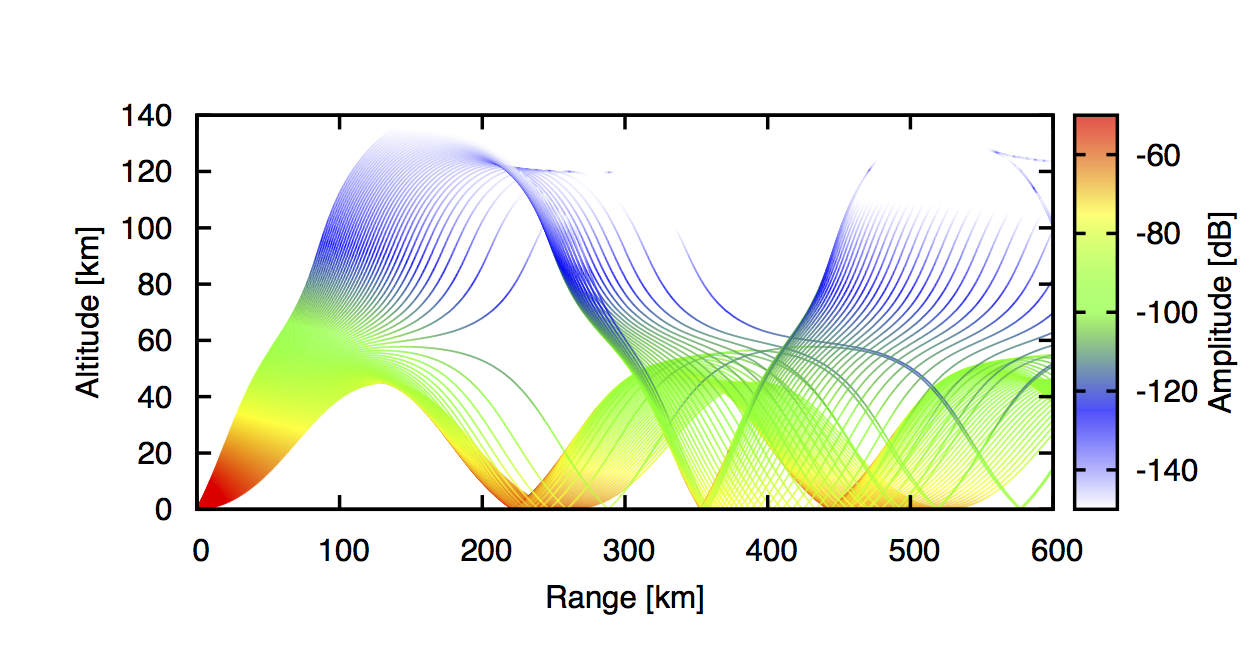
\includegraphics[width=0.75\textwidth]{Figures/2DExample1.png}}
\caption[Ray Path Figure]{Example ray path figure generated with GNUPlot commands.}
\end{figure}

\begin{figure}
\centering
\boxed{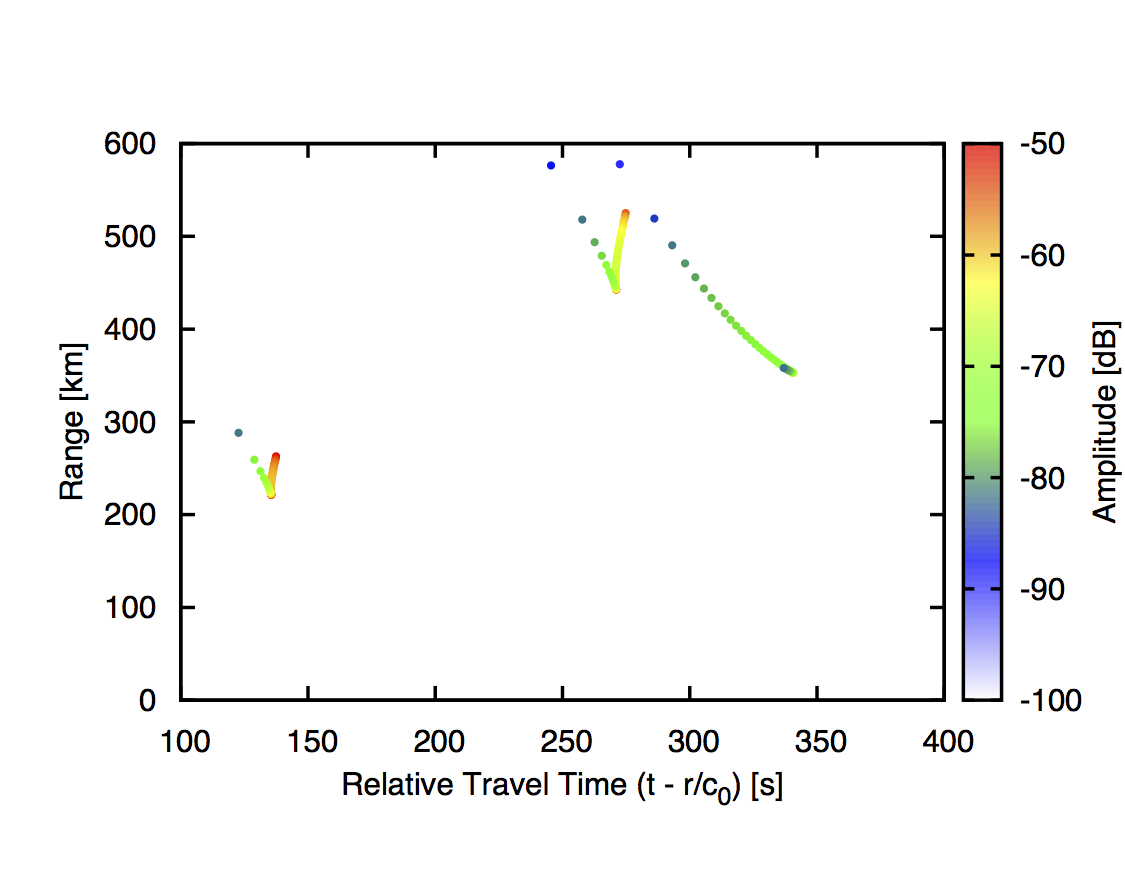
\includegraphics[width=0.5\textwidth]{Figures/2DExample2.png}}
\caption[Travel Time Figure]{Relative travel time figure generated with GNUPlot commands.}
\end{figure}

\begin{figure}
\centering
\boxed{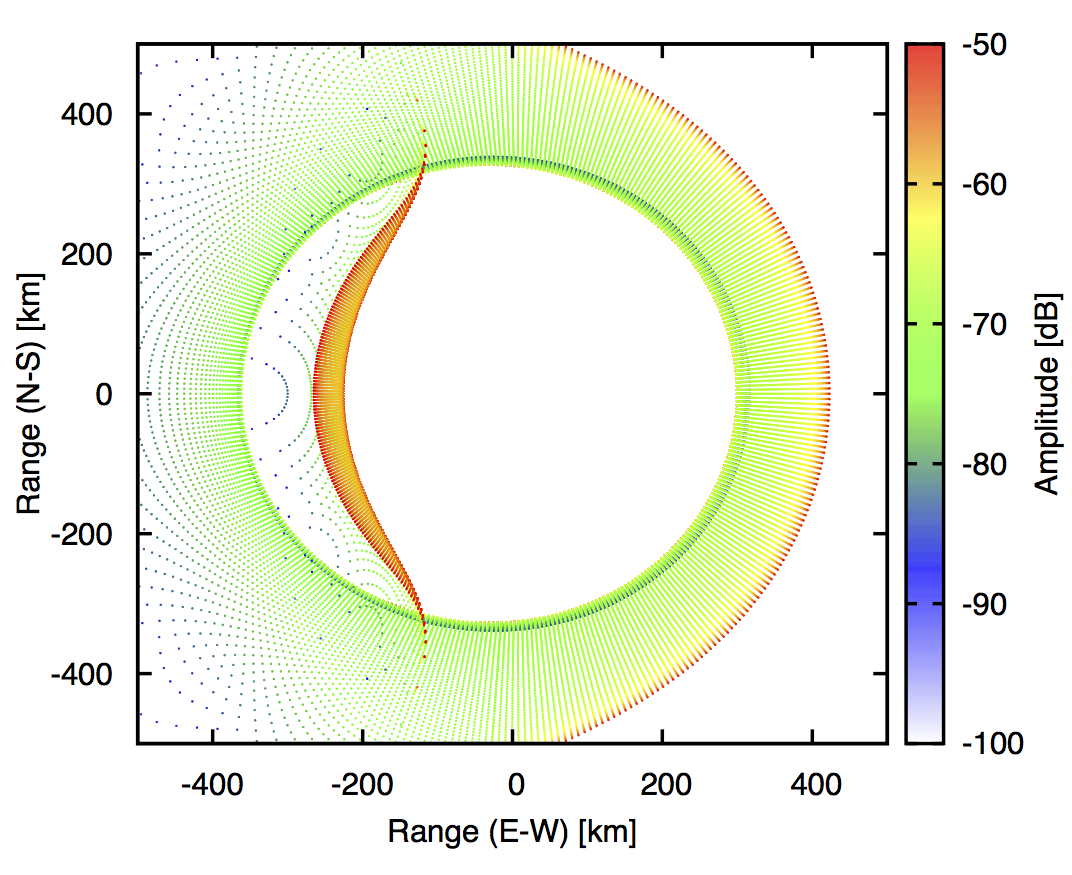
\includegraphics[width=0.48\textwidth]{Figures/3DExample1.png}}
\boxed{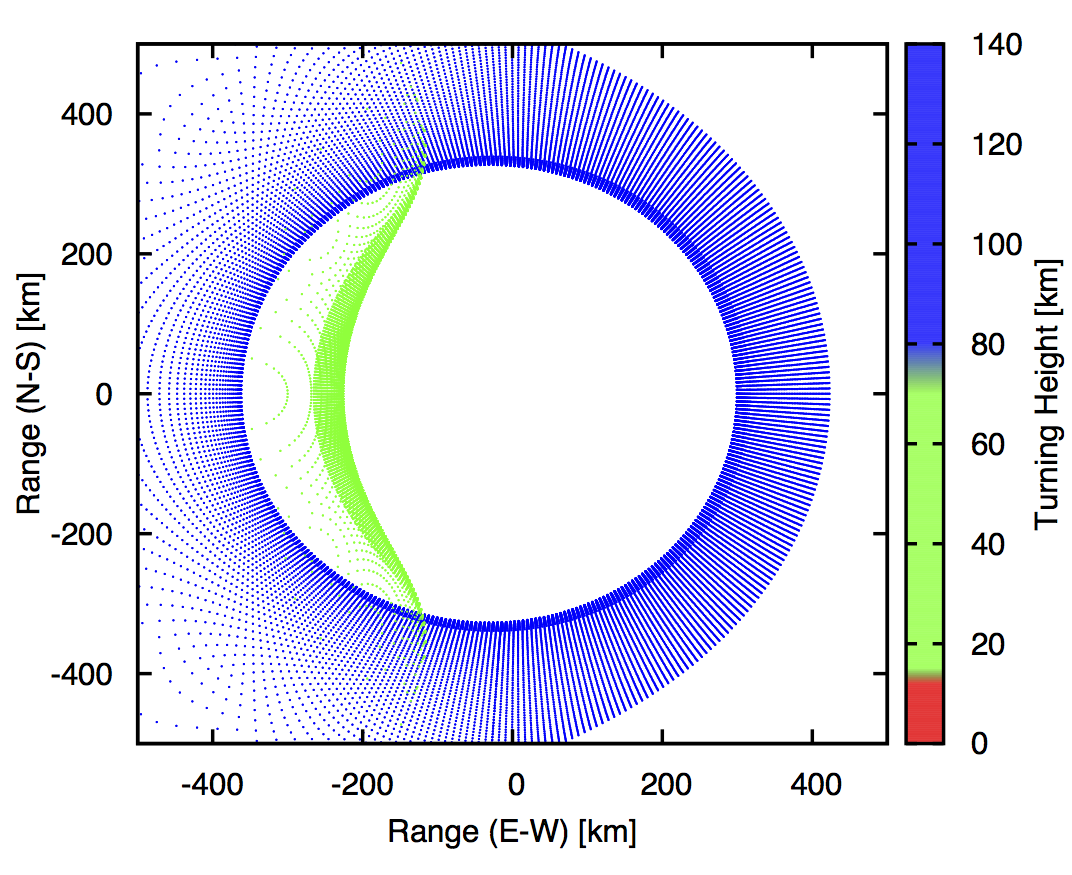
\includegraphics[width=0.48\textwidth]{Figures/3DExample2.png}}
\caption[Travel Time Figure]{Arrival amplitudes and turning heights for 3D propagation.  Similar results for global case.}
\end{figure}

\newpage
\section{Mathematical Background - What Does infraGA Do?}

The propagation of acoustic energy can be described by a linear perturbation of the fluid mechanics equations.  The linear order continuity, Euler, and state equations for an inhomogeneous, moving medium have the forms,
\begin{subequations}
\label{Eq:LinearizedGeometric}
\begin{equation}
 \label{Eq:LinearizedGeometric:MassConservation}
 \frac{D \rho}{D t} + \rho \vec{\nabla} \cdot \vec{v}_0 + \vec{\nabla} \cdot \left( \rho_0 \vec{v} \right) = 0,
\end{equation}
\begin{equation}
 \label{Eq:LinearizedGeometric:MomentumConservation}
\frac{D \vec{v}}{Dt}  + \left( \vec{v} \cdot \vec{\nabla} \right) \vec{v}_0 = -\frac{1}{\rho_0} \vec{\nabla} p + \rho \vec{\nabla} \frac{p_0}{\rho_0^2},
\end{equation}
\begin{equation}
 \label{Eq:LinearizedGeometric:State}
 \vec{v} \cdot \vec{\nabla} p_0 + \frac{D p}{D t} = c^2 \left[ \vec{v} \cdot \vec{\nabla} \rho_0 + \frac{D \rho}{D t} \right] + \left( c^2 \right)^\prime \vec{v}_0 \cdot \vec{\nabla} \rho_0,
\end{equation}
\end{subequations}
where subscript \(0\)'s denote ambient quantities that vary in space and those without subscripts denote acoustic perturbations that vary in space and time.  The approximation of geometric acoustics is constructed by expanding each variable with a spatially varying phase, \(e^{i k_0 \lambda \left( \vec{x} \right)}\), and Debye series, \(\sum{ \frac{\mathcal{P}_j (\vec{x})}{(i k_0)^j}}\).  The phase function, \(\psi \left( \vec{x} \right)\), is termed the Eikonal and its solution provides information about the deformation of surfaces of constant phase.  Expanding each linear variable,
\begin{equation}
 \label{Eq:GeometricExpansion}
\begin{pmatrix}
p \\ \vec{v} \\ \rho \\ \left( c^2 \right)^\prime
\end{pmatrix} =
e^{i k_0 \lambda \left( \vec{x} \right)} \sum_{j = 0}^\infty{\frac{1}{\left( i k_0 \right)^j}
\begin{pmatrix}
 \mathcal{P}_j \left( \vec{x} \right) \\
 \vec{\mathcal{V}}_j \left( \vec{x} \right) \\
 \mathcal{D}_j \left( \vec{x} \right) \\
 \mathcal{C}_j \left( \vec{x} \right)
\end{pmatrix}}.
\end{equation}
The linearized fluid mechanics equations can then be written as,
\begin{small}
\begin{subequations}
 \begin{align}
  & \sum_{j = 0}^\infty{\frac{1}{\left( i k_0 \right)^j} \Big\{ -i k_0 \mathcal{D}_j \left( c_0  - \vec{v}_0 \cdot \vec{\psi} \right) + \vec{v}_0 \cdot \vec{\nabla} \mathcal{D}_j + \mathcal{D}_j \vec{\nabla} \cdot \vec{v}_0} + \rho_0 \vec{\nabla} \cdot \vec{\mathcal{V}}_j + \rho_0 i k_0 \vec{\mathcal{V}}_j \cdot \vec{\psi} + \vec{\mathcal{V}}_j \cdot \vec{\nabla} \rho_0 \Big\} = 0,
 \end{align}
 \begin{align}
  &\sum_{j = 0}^\infty{\frac{1}{\left( i k_0 \right)^j} \left\{ -i k_0 \vec{\mathcal{V}}_j \left( c_0 - \vec{v}_0 \cdot \vec{\psi} \right) + \vec{v}_0 \cdot \vec{\nabla} \vec{\mathcal{V}}_j + \vec{\mathcal{V}}_j \cdot \vec{\nabla} \vec{v}_0 \right\}} = \sum_{j = 0}^\infty{\frac{1}{\left( i k_0 \right)^j}  \left\{ -  \frac{i k_0}{\rho_0}  \mathcal{P}_j   \vec{\psi} - \frac{1}{\rho_0} \vec{\nabla} \mathcal{P}_j  + \mathcal{D}_j \vec{\nabla} \frac{p_0}{\rho_0{}^2} \right\} },
 \end{align}
 \begin{align}
  & \sum_{j = 0}^\infty{\frac{1}{\left( i k_0 \right)^j} \left\{ \vec{\mathcal{V}}_j \cdot \vec{\nabla} p_0 - i k_0 \mathcal{P}_j \left( c_0 -  \vec{v}_0 \cdot \vec{\psi} \right) + \vec{v}_0 \cdot \vec{\nabla} \mathcal{P}_j \right\} } \nonumber  \\
  & \hspace{0.2\textwidth} = \sum_{j = 0}^\infty{\frac{1}{\left( i k_0 \right)^j} \Big\{ c^2 \left[ \vec{\mathcal{V}}_j \cdot \vec{\nabla} \rho_0  -i k_0 \mathcal{D}_j \left( c_0 - \vec{v}_0 \cdot \vec{\psi} \right) + \vec{v}_0 \cdot \vec{\nabla} \mathcal{D}_j \right]} + \mathcal{C}_j \vec{v}_0 \cdot \vec{\nabla} \rho_0 \Big\},
\end{align}
\end{subequations}
\end{small}
where we've defined \(\vec{\psi} = \vec{\nabla} \lambda\).  Collecting terms in powers of \(k_0\), the leading order contributions require
\begin{subequations}
 \label{Eq:EikonalEqs}
\begin{align}
 \label{Eq:EikonalEqs:MassConservation}
\left( 1 - \frac{\vec{v}_0 \cdot \vec{\psi}}{c_0} \right) \mathcal{D}_0 & = \frac{\rho_0}{c_0} \vec{\mathcal{V}}_0 \cdot \vec{\psi}, \\
 \label{Eq:EikonalEqs:Euler}
\left( 1 - \frac{\vec{v}_0 \cdot \vec{\psi}}{c_0} \right) \vec{\mathcal{V}}_0 & = \frac{1}{\rho_0 c_0} \mathcal{P}_0 \vec{\psi},  \\
 \label{Eq:EikonalEqs:State}
 \mathcal{P}_0 & = c^2 \mathcal{D}_0,
 \end{align}
\end{subequations}
which can be combined to obtain the Eikonal Equation,
\begin{equation}
 \psi^2 = \frac{c_0^2}{c^2 \left( \vec{x} \right) } \left[ 1 - \frac{\vec{v}_0 \left( \vec{x} \right) \cdot \vec{\psi}}{c_0} \right]^2.
\end{equation}

In addition to the ray path geometry defined by the Eikonal Equation, higher order terms in the expansion provide a means to estimate ray spreading and geometric attenuation.  Taking the terms in the expansion proportional to \(k_0\),
\begin{subequations}
 \label{Eq:TransportEqs}
\begin{align}
& \left( 1 - \frac{\vec{v}_0 \cdot \vec{\psi}}{c_0} \right) \vec{\mathcal{V}}_1 - \frac{1}{\rho_0 c_0} \mathcal{P}_1 \vec{\psi} \nonumber \\
 \label{Eq:TransportEqs:Continuity}
& \hspace{0.2\textwidth} =  \frac{1}{c_0} \left[ \vec{v}_0 \cdot\vec{\nabla}\vec{\mathcal{V}}_0 + \vec{\mathcal{V}}_0 \cdot\vec{\nabla}\vec{v}_0 + \frac{1}{\rho_0} \vec{\nabla} \mathcal{P}_0 - \frac{\mathcal{D}_0}{\rho_0{}^2}\vec{\nabla}p_0 \right] = \vec{b}, \\
 \label{Eq:TransportEqs:Euler}
&\left( 1 - \frac{\vec{v}_0 \cdot \vec{\psi}}{c_0} \right) \mathcal{D}_1 - \frac{\rho_0}{c_0} \vec{\psi} \cdot \vec{\mathcal{V}}_1 = \frac{1}{c_0}\vec{\nabla}\cdot \left( \mathcal{D}_0 \vec{v}_0 + \rho_0 \vec{\mathcal{V}}_0 \right) = b_1, \\
 \label{Eq:TransportEqs:State}
&\mathcal{P}_1 - c^2 \mathcal{D}_1 = \frac{1}{c \psi} \left[ \vec{\mathcal{V}}_0 \cdot\vec{\nabla} p_0 + \vec{v}_0 \cdot\vec{\nabla}\mathcal{P}_0 - c^2 \vec{v}_0 \cdot\vec{\nabla} \mathcal{D}_0 - \frac{\mathcal{P}_0}{c^2} \vec{v}_0 \cdot \vec{\nabla} c^2 - c^2 \vec{\mathcal{V}}_0 \cdot\vec{\nabla}\rho_0 \right] = b_2,
\end{align}
\end{subequations}
Using the Eikonal Equation condition, these equations can be combined in a manner which goes to zero,
\begin{equation}
\left\{
\begin{matrix}
\psi \vec{\mathcal{V}}_1 - \frac{1}{\rho_0 c_0} \mathcal{P}_1 \vec{\psi} = \vec{b} \\ \\
\psi \mathcal{D}_1 - \frac{\rho_0}{c_0} \vec{\psi} \cdot \vec{\mathcal{V}}_1 = b_1 \\ \\
\mathcal{P}_1 - c^2 \mathcal{D}_1 = b_2
\end{matrix}
\right. \quad \quad \rightarrow \quad
\frac{c_0 \rho_0}{\psi} \vec{\psi} \cdot \vec{b} + c_0 c b_1 + \psi b_2 = 0.
\end{equation}
Solving this condition leads to the transport equation,
\begin{equation}
 \label{Eq:TransportEq}
\vec{\nabla} \cdot \left( \mathcal{P}_0^2 \vec{c}_g \right) = \mathcal{P}_0^2 \vec{c}_g \cdot \vec{\nabla} \ln \left( \rho_0 c^3 \psi \right),
\end{equation}
and the resulting amplitude term is defined in terms of the Jacobian, \(D \left( s, \vartheta, \varphi \right)\) where \(s\), \(\vartheta\), and \(\varphi\) are the ray length, initial inclination angle, and initial azimuthal angle of the ray path respectively, that describes the coordinate transformation between Cartesian and ray coordinates, 
\begin{equation}
  \mathcal{P}_0 \left( s, \vartheta, \varphi \right) = \frac{1}{4 \pi} \left| \frac{\rho_0 \left( s \right) \psi \left( s \right) c^3 \left( s \right)}{\rho_0 \left( 0 \right) \psi \left( 0 \right) c^3 \left( 0 \right)} \frac{c_g \left( 0 \right) \,  \cos \vartheta}{c_g \left( s \right) D \left( s, \vartheta, \varphi \right) } \right|^\frac{1}{2}.
\end{equation}
Spherical spreading at the source has been assumed so that \(\mathcal{P}_0 \left( s, \vartheta, \varphi \right)|_{s \downarrow 0} = \frac{1}{4\pi s^2}\) and \(D \left( s, \vartheta, \varphi \right)|_{s \downarrow 0} = s^2 \cos \vartheta \), 

The Eikonal Equation can be used to define a Hamiltonian, \(  H \left( \vec{x}, \vec{\psi} \right) = 0 \) and the Hamilton-Jacobi relations used to define equations governing ray paths,
 \begin{equation}
 \label{Eq:EikonalHamiltonJacobi:DEs}
  \frac{\partial \vec{x}}{\partial \tau} = \frac{\partial H}{\partial \vec{\psi}}, \quad \quad
  \frac{\partial \vec{\psi}}{\partial \tau} = - \frac{\partial H}{\partial \vec{x}}.
 \end{equation}
 For the methods in infraGA, the parameter \(\tau\) is replaced by ray length, \(s\), such that \(\left| d \vec{x} \right| = ds \).  The transport coefficient depends on the Jacobian determinant which is defined by the variation between coordinate systems.  Denoting the initial launch inclination and azimuth as \(\vartheta\) and \(\varphi\), respectively, one has,
 \begin{equation}
 D \left( x, y, z; s, \vartheta, \varphi \right) = \left| \frac{\partial \left( x, y, z \right)}{\partial \left( s, \vartheta, \varphi \right)} \right| = 
\textbf{det} \begin{pmatrix}
  \frac{\partial x}{\partial s} && \frac{\partial x}{\partial \vartheta} && \frac{\partial x}{\partial \varphi} \\ \\
  \frac{\partial y}{\partial s} && \frac{\partial y}{\partial \vartheta} && \frac{\partial y}{\partial \varphi} \\ \\
  \frac{\partial z}{\partial s} && \frac{\partial z}{\partial \vartheta} && \frac{\partial z}{\partial \varphi}
 \end{pmatrix} 
 \end{equation}
  As detailed in Blom \& Waxler (2012), the \(s\) derivatives can be defined directly from the Eikonal Equation condition, but the \(\vartheta\) and \(\varphi\) derivatives require the introduction of auxiliary parameters, \(\mathcal{X}^{(\vartheta)} = \frac{\partial x}{\partial \vartheta}\), \(\mathcal{X}^{(\varphi)} = \frac{\partial x}{\partial \varphi}\) with similar parameters defined for \(\mathcal{Y}\) and \(\mathcal{Z}\).

\newpage

\subsection{Propagation in two-dimensions using the effective sound speed}

In the case of the effective sound speed approximation, one re-defines \(c \rightarrow c + \vec{v}_0 \cdot \hat{\psi}_\perp\) (adding the wind in the direction of propagation to the adiabatic sound speed) and \(\vec{v} = 0\) in the relations.  This reduces the Eikonal to, \(\psi^2 = \frac{c_0^2}{c^2}\), and the propagation relations become simply,
\begin{subequations}
 \begin{align}
 \frac{\partial \vec{x}}{\partial s} &= \frac{c_0}{c} \vec{\psi} , \quad \quad \frac{\partial \psi_j}{\partial s} = - \frac{c_0}{c^2} \frac{\partial c}{\partial x_j} ,
 \end{align}
\end{subequations}



\subsection{Propagation in three-dimensions using an inhomogeneous moving medium}
The differential equations describing the geometric ray paths in an arbitrary moving medium can be found from the Eikonal derived above,
\begin{subequations}
 \begin{align}
 \frac{\partial \vec{x}}{\partial s} &= \frac{\vec{c}_g}{c_g}, \quad \vec{c}_g = c \frac{\vec{\psi}}{\psi} + \vec{v}_0 \\
 \frac{\partial \psi_j}{\partial s} & = - \frac{1}{c_g} \left[ \psi \frac{\partial c}{\partial x_j} + \vec{\psi} \cdot \frac{\partial \vec{v}_0}{\partial x_j} \right].
 \end{align}
\end{subequations}
This is the equation set used in the \verb=infraga-3d= methods.


\subsection{Propagation in spherical coordinates}

The eikonal solution in spherical coordinates has been derived and can be summarized as,
 \begin{subequations}
\label{Eq:Curvilinear}
 \begin{align}
 \frac{\partial u_j}{\partial s} & = \mathcal{G}_j\frac{c_{g,j}}{c_g} , \quad \quad c_{g,j} = c \frac{\psi_j}{\psi} + v_j,\\
  \frac{\partial \psi_j}{\partial s} & = - \frac{\mathcal{G}_j}{c_g} \left( \psi \frac{\partial c}{\partial u_j} + \sum_k{ \psi_k \frac{\partial v_k}{\partial u_j}} + \mathcal{T}_j \right),
  \label{Eq:Curvilinear:r}
 \end{align}
 where geometric scaling coefficients and corrective terms for the spatial variability of the spherical coordinate unit vectors produce,
\begin{align}
 \mathcal{G}_r & = 1,  \quad 
 \mathcal{G}_\theta = \frac{1}{r}, \quad
 \mathcal{G}_\phi = \frac{1}{r \cos \theta}, \\
 \mathcal{T}_r & =  \frac{1}{r} \left( \psi_\theta c_{g,\theta} + \psi_\phi  c_{g,\phi} \right),   \\
 \mathcal{T}_\theta & =  \left( \psi_r v_\theta - \psi_\theta v_r \right) - \left( \psi_r c_{g,\theta} - \psi_\phi  c_{g,\phi}  \tan \theta \right),  \\
 \mathcal{T}_\phi & =  \left( \psi_r v_\phi - \psi_\phi v_r \right) \cos \theta \nonumber \\
 & \hspace*{25pt} + \left( \psi_\theta v_\phi - \psi_\phi v_\theta \right) \sin \theta \nonumber \\
 & \hspace*{50pt} - c_{g,\phi} \left( \psi_r \cos \theta + \psi_\theta \sin \theta \right).
\end{align}
 \end{subequations} 
 This is the equation set used in the \verb=infraga-sph= methods.

\subsection{Eigenray methods}

Eigenrays are identified using the auxiliary parameters defined in order to compute the Jacobian components needed to calculate geometric spreading.  Considering the arrival location of a ray path in 3D,
\begin{subequations}
\begin{align}
 x_0 \left( \theta + \delta \theta, \phi + \delta \phi \right) = x_0 \left( \theta, \phi \right) + \frac{\partial x_0}{\partial \theta} \delta \theta + \frac{\partial x_0}{\partial \phi} \delta \phi + O \left( \delta^2 \right),  \\
 y_0 \left( \theta + \delta \theta, \phi + \delta \phi \right) = y_0 \left( \theta, \phi \right) + \frac{\partial y_0}{\partial \theta} \delta \theta + \frac{\partial y_0}{\partial \phi} \delta \phi + O \left( \delta^2 \right),
\end{align}
This can be written more compactly as,
\begin{equation}
\begin{pmatrix}
  \delta x_0 \\
  \delta y_0  
 \end{pmatrix} = 
  \begin{pmatrix}
 \frac{\partial x_0}{\partial \theta} & \frac{\partial x_0}{\partial \phi} \\
 \frac{\partial y_0}{\partial \theta} & \frac{\partial y_0}{\partial \phi}
 \end{pmatrix}
 \begin{pmatrix}
 \delta \theta \\ \delta \phi
 \end{pmatrix},
\end{equation}
or simply,
\begin{equation}
 \delta \vec{x}_0 = \bm{\mathcal{D}}_0 \, \delta \vec{\vartheta}.
\end{equation}
From this linear approximation, a Levenberg-Marquardt algorithm can be constructed,
\begin{equation}
\label{Eq:EigLM}
 \delta \vec{\vartheta} = \left( \bm{\mathcal{D}}_0 + \lambda  \text{ diag} \left(\bm{\mathcal{D}}_0 \right) \right)^{-1} \delta \vec{x}_0,
\end{equation}
that will identify the changes in ray launch angles, \(\delta \vec{\vartheta}\) needed to shift the arrival location by some distance, \(\delta \vec{x}_0\).  This algorithm is utilized as a stand alone method in \verb=-eig_direct= and as the precision search step in \verb=-eig_search= where a preliminary inclination/range search is used to identify initial solutions near eigenrays.
\end{subequations}

\subsection{Ground reflections and topography}

The reflection conditions for including topography are modified so that the eikonal vector components along the ground surface are conserved and the normal component to the ground changes sign,
\begin{equation}
 \vec{\psi}_\text{refl} \cdot \hat{n}_\text{grnd} = - \vec{\psi}_0 \cdot \hat{n}_\text{grnd}, \quad
 \vec{\psi}_\text{refl} \times \hat{n}_\text{grnd} = \vec{\psi}_0 \times \hat{n}_\text{grnd}.
\end{equation}
where \(\vec{\psi}_0\) denotes the incident eikonal vector.  The resulting reflection conditions can then be defined by relating the ground normal to the derivative of the functional ground surface specification, \(z_g \left( x, y \right)\),
\begin{subequations}
 \begin{align}
  \psi_x \left( s_0 + 0^+, \vartheta, \varphi \right) & = \mathcal{C}_1^{(x)}  \psi_{x,0} + \mathcal{C}_2^{(x)} \left( \psi_{z,0} - \psi_{y,0} \frac{\partial z_g}{\partial y} \right), \\
  \psi_y \left( s_0 + 0^+, \vartheta, \varphi \right) & = \mathcal{C}_1^{(y)}  \psi_{y,0} + \mathcal{C}_2^{(y)} \left( \psi_{z,0} - \psi_{x,0} \frac{\partial z_g}{\partial x} \right), \\
  \psi_z \left( s_0 + 0^+, \vartheta, \varphi \right) & = -\mathcal{C}_1^{(z)} \psi_{z, 0} + \mathcal{C}_2^{(x)} \psi_{x,0} + \mathcal{C}_2^{(y)} \psi_{y,0}.
 \end{align}
where,
\begin{align*}
\mathcal{C}_1^{(x)} & = \frac{1 - \left(\frac{\partial z_g}{\partial x} \right)^2 + \left(\frac{\partial z_g}{\partial y} \right)^2}{1 + \left(\frac{\partial z_g}{\partial x} \right)^2 + \left(\frac{\partial z_g}{\partial y} \right)^2}, & 
\mathcal{C}_2^{(x)} &= \frac{2 \frac{\partial z_g}{\partial x}}{1 + \left(\frac{\partial z_g}{\partial x} \right)^2 +\left(\frac{\partial z_g}{\partial y} \right)^2}, \\
\mathcal{C}_1^{(y)} & =\frac{1 + \left(\frac{\partial z_g}{\partial x} \right)^2 - \left(\frac{\partial z_g}{\partial y} \right)^2}{1 + \left(\frac{\partial z_g}{\partial x} \right)^2 + \left(\frac{\partial z_g}{\partial y} \right)^2}, & 
\mathcal{C}_2^{(y)} &= \frac{2 \frac{\partial z_g}{\partial y}}{1 + \left(\frac{\partial z_g}{\partial x} \right)^2 +\left(\frac{\partial z_g}{\partial y} \right)^2}, \\
\mathcal{C}_1^{(z)} & = \frac{1 - \left(\frac{\partial z_g}{\partial x} \right)^2 - \left(\frac{\partial z_g}{\partial y} \right)^2}{1 + \left(\frac{\partial z_g}{\partial x} \right)^2 + \left(\frac{\partial z_g}{\partial y} \right)^2}.
\end{align*}
\end{subequations}


\subsection{Weakly non-linear waveform calculation}

The waveform evolution is computed using the methods developed by Lonzaga \textit{et al.} (2015) using a Heun's solver (RK2).  The equations being solved are,
\begin{subequations}
\begin{equation}
\frac{\partial u}{\partial s} = \tilde{\beta} u \frac{\partial u}{\partial \tau}, \quad 
\tilde{\beta} \left( s\right) = \beta \frac{p_0}{\rho_0 c_0^2} \frac{\psi_0 c_0}{c_{g,0} c_\text{src}} \sqrt{ \frac{D_0 \rho_0 c_{g,0}^3}{D \rho c_g^3} \frac{c \psi^3}{c_0 \psi_0^3}},
\end{equation}
\begin{equation}
 u \left( s, \tau \right) = \frac{p \left( s, \tau \right)}{p_\text{ref}} \sqrt{ \frac{\rho_0 c_0^3 \psi_0}{\rho c^3 \psi} \frac{c_{g} D}{c_{g,0} D_0}},
\end{equation}
\end{subequations}
where subscript zeros denote evaluation at some reference point, \(s = s_0\), along the ray path.  The variable step size in the solver is defined as \(ds = ds_0 /  \left( \pi \tilde{\beta} \left( s \right) \text{max} \left(\mathcal{U} \left( s, f \right) \right) \right)\), where \(\mathcal{U} \left( s, f \right)\) is the FFT of \(u \left(s, t \right)\) along the ray path and \(ds_0\) is defined in the code as \verb=wvfrm_ds=.  

In cases for which little energy is expected hear the Nyquist frequency, a value of \(ds_0 \sim1.0\) can be used; however, for source waveforms with high frequency content (e.g., a blast wave) or propagation paths extending into the upper atmosphere where rarefaction leads to strong relatively strong non-linear effects and generation of high frequency energy, a value of \(\sim0.1\) might be required.  Best practice is to vary the value of \verb=wvfrm_ds= to be sure your analysis has converged.


\newpage
\section{Acknowledgement of Use}
The algorithms included in \verb=infraGA/GeoAc= have been documented in a number of peer reviewed publications and the authors request that others acknowledge of the use of the methods in published research by citing the appropriate manuscript(s) below for the various methodologies.
\begin{itemize}
  \item Blom, P. \& Waxler, R. (2012). ``Impulse propagation in the nocturnal boundary layer: Analysis of the geometric component". \textit{J. Acoust. Soc. Am.}, \textbf{131}(5), 3680 -- 3690 .
  \item Blom, P. \& Waxler, R. (2017). ``Modeling and observations of an elevated, moving infrasonic source: eigenray methods". \textit{J. Acoust. Soc. Am.}, \textbf{141}(4), 2681--2692.
  \item Blom, P. (2019). ``Modeling infrasonic propagation through a spherical atmospheric layer: Analysis of the stratospheric pair." \textit{J. Acoust. Soc. Am.}, \textbf{145}(4), 2198--2208.	
  \item Blom, P. \& Waxler, R. (2020). ``Characteristics of thermospheric infrasound predicted using ray tracing and weakly non-linear waveform analysis" \textit{J. Acoust. Soc. Am.}, in peer review.	
  \item Blom, P. (2020). ``The influence of irregular terrain on infrasonic propagation in the troposphere" \textit{J. Acoust. Soc. Am.}, in peer review.	
\end{itemize}

\section{Citations}
The ray tracing methods developed as well as many of the other underlying methods in \verb=infraGA/GeoAc= leveraged work by many researchers including those below.
\begin{itemize}
  \item Brekhovskikh, L. M., \& Godin, O. (2013).  \textit{Acoustics of layered media II: point sources and bounded beams} (Vol. 10). Springer Science \& Business Media.
  \item Keys, R. G. (1981). ``Cubic convolution interpolation for digital image processing." \textit{Acoustics, Speech and Signal Processing, IEEE Transactions on}, \textbf{29}(6), pp. 1153-1160.
  \item Lonzaga, J. B., Waxler, R. M., Assink, J. D., \& Talmadge, C. L. (2015). ``Modelling waveforms of infrasound arrivals from impulsive sources using weakly non-linear ray theory." \textit{Geophysical Journal International}, \textbf{200}(3), 1347-1361.
  \item Pierce, A. D. (1980).  \textit{Acoustics: An introduction to its physical principles and applications.}  McGraw-Hill Inc. 

  \item Sutherland, L. C., \& Bass, H. E., (2004). Atmospheric absorption in the atmosphere up to 160 km. \textit{The Journal of the Acoustical Society of America}, \textbf{115}(3), pp.1012-1032.

 \end{itemize}







\end{document}
